%---------- Inleiding ---------------------------------------------------------

\section{Introductie}%
\label{sec:introductie}

Augmented reality, of kortweg AR, omvat een samensmelting van de virtuele wereld met de echte wereld door middel van een overlay.
Deze technologie bestaat voornamelijk in twee vormen: mobiele AR, die inmiddels al een wijde aanneming kent volgens een onderzoek van \textcite{Berggren2023}, en head-mounted AR.
Voor de voorgaande vorm biedt Tropos AR een out of the box user interface (UI) aan via haar Troposphere software-development kit (SDK).
Mobiele AR-ontwikkelaars hoeven hierdoor niet langer de focus te leggen op interacties van gebruikers met de AR-wereld, waardoor ontwikkelingstijd aanzienlijk verkleind kan worden.

Head-mounted Augmented Reality daarentegen kende meer technischere obstakels waardoor er tot recentelijk geen consument-gerichte modellen op de markt waren.
2023 kende echter een opkomst van dit soort modellen, onder de vorm van de Meta Quest 3 en de aankondiging van de Apple VisionPro.
Met de influx van deze head-mounted devices komt ook het ontstaan van een nieuwe markt waar Tropos AR op wilt inspelen.

Hoewel Tropos AR reeds knowhow opgebouwd heeft van bestaande UI-technieken binnen AR op smartphones, kunnen deze niet altijd even goed vertaald worden naar head-mounted AR.
Concreet is Tropos AR op zoek naar een manier om bestaande mobiele AR-ervaringen te vertalen naar deze nieuwe, opkomende vorm.
Ook is er vraag naar de verschillende manieren om een menu af te beelden en hierbinnen te navigeren.
Deze thesis probeert hier antwoorden voor te voorzien aan de hand van een rapport met aanbevelingen.

%---------- Stand van zaken ---------------------------------------------------

\section{Literatuurstudie}%
\label{sec:state-of-the-art}

\subsection{Het ontstaan van (mobiele) AR}
\label{subsec:wat-is-ar}
Met haar eerste iteratie in de vorm van een head-mounted display ontwikkeld door \textcite{Sutherland1968} , kende Augmented Reality een opmerkelijke voorsprong op de hedendaagse smartphone.
Toch kent deze vorm van AR niet dezelfde aanneming door het algemene publiek en is tot recentelijk enkel een vorm van mobiele AR (gebruikmakend van smartphones) aanwezig op de markt.

Head-mounted AR had vooral te lijden aan grotere technologische obstakels zoals de displays waarop een samensmelting van de virtuele met de echte wereld geprojecteerd wordt \autocite{YunHan2019} .
Hierdoor was het aan koplopers zoals Meta en Varjo om aanzienlijke budgetten te besteden om deze obstakels te kunnen overbruggen en de fundamenten van deze markt tot stand te krijgen. % TODO miss bron?
Intussen zagen smartphonemakers zoals Samsung en Apple een opportuniteit om deze technologie toch in de handen te zien krijgen bij consumenten, dit in de vorm van mobiele AR.
Zo bepalen hedendaagse smartphones met behulp van camera's en sensoren de plaats van digitale entiteiten en tonen ze deze vervolgens op hun scherm.

\subsection{Head-mounted AR en gebaren}
\label{subsec:ar-gestures}
Head-mounted AR is een radicaal andere ervaring van de samensmelting van virtueel met fysiek: in tegenstelling tot mobiele AR neemt deze vorm van AR heel het gezichtsveld in beslag.
Hierdoor verdwijnt echter ook de on-screen navigatie die men vandaag de dag gewend is aan smartphones en wordt deze vervangen met gebaren.

Een mogelijk alternatief hiervoor is om via gebaren te interageren met virtuele objecten, een alternatief waar Apple vooral op zal steunen met haar Vision Pro model.
De werking hiervan wordt bepaald door middel van camera's die de posities van de gebruikers' handen bepaalt en vertaalt naar interacties met menu's \textcite{Shrestha2018} .
Uit onderzoek van \textcite{Datcu2013} blijkt dat deze manier van virtuele objecten en menu's te besturen de voorkeur kent bij gebruikers.

\subsection{Het voordeel van head-mounted devices}
\label{subsec:benefits-hmd}
Head-mounted devices maken het mogelijk voor de gebruiker om direct aan de slag te gaan met de virtuele wereld zonder hierbij een telefoon vast te houden.
Het gevoel van kijken door een soort venster verdwijnt doordat de samensmeltende werelden direct geprojecteerd worden in de ogen van gebruikers.
Deze categorie van AR-apparaten krijgt daardoor vaak de term \("\)Immersive AR\("\) en kent ook vandaag al een meerwaarde in onder andere de medische sector tijdens het opleiden van chirurgen~\autocite{Waisberg2023} .

%---------- Methodologie ------------------------------------------------------
\section{Methodologie}%
\label{sec:methodologie}
\subsection{Voorafgaande literatuurstudie}
\label{subsec:literature-study}
In de eerste fase vindt zich een voorafgaande literatuurstudie over het onderwerp plaats. % 2 weken
Het praktische doel hiervan is om een verdere inzicht te krijgen op de werking van gesture-gebaseerde navigatie in head-mounted devices.
De nadruk ligt hierbij op de evolutie van deze werking en het verschil van hedendaagse mobiele AR-besturing.
Tijdens deze fase komen de gelijkenissen en verschillen tussen de twee werkwijzes om tijdens de derde fase met elkaar te kunnen verzoenen naar voren.

\subsection{Requirements-analyse}
\label{subsec:requirements-analysis}
Vervolgens vindt er zich een requirements-analyse plaats bij Tropos AR over de gewenste interactiemogelijkheden binnen Immersive AR. % 3 weken
Ook klanten van de Tropos AR SDK zullen participeren aan een bevraging, met als richtlijn waarom ze specifiek gekozen hebben voor de Tropos framework.
Uit deze bevraging blijkt een lijst van gewenste resultaten waar een proof-of-concept zich op zal richten, deze wordt opgesteld aan de hand van de MoSCoW-methode.
Deze lijst bevat enerzijds de visie van Tropos AR voor interacties met virtuele objecten.
Anderzijds bevat deze een blik op bestaande mobiele AR-applicaties en hoe de ontwikkelaars hun functionaliteiten wensen gebruikt te zien worden door consumenten.

\subsection{Proof-of-concept}
\label{subsec:poc}
Gedurende de derde fase wordt een applicatie gebouwd op de Troposhere SDK geselecteerd. % 5 weken
Belangrijk hierbij is dat deze applicatie voldoende verschillende interactiemogelijkheden bevat die tijdens de requirements-analyse aan het licht kwamen.
Subsequent worden de user interface-elementen van de interacties vertaald naar gesture-geoptimaliseerde versies in de vorm van een proof-of-concept.
Gezien Troposphere (en dus ook haar toepassingen) beschikbaar is op Android en gebruik maakt van de Unity game-engine, lijkt de Meta Quest 3 voor de hand liggend als platform voor de proof-of-concept.
Dit AR-apparaat is de eerste toegankelijke versie van een AR head-mounted device voor het algemeen publiek en maakt tevens ook gebruik van deze technologie\"en.
Hierdoor kan de originele code van de applicatie bewaard blijven en hoeven enkel de functionaliteiten van de SDK vertaald te worden.
De proof-of-concept toetst de mogelijke antwoorden die tijdens de literatuurstudie aan bod kwamen op de requirements af.

\subsection{Rapport met aanbevelingen}
\label{subsec:result-of-poc}
Na het opzetten van de proof-of-concept komen enkele gebruikerstests aan bod. % 3 weken
Hierbij worden het gebruikspatroon en de tijdsduur en foutenpercentage voor het uitvoeren van taken vastgelegd.
Een analyse van deze cijfers zal de bruikbaarheid van de voorgestelde oplossingen aantonen.
Daaropvolgend wordt een rapport met aanbevelingen opgesteld voor Tropos AR.

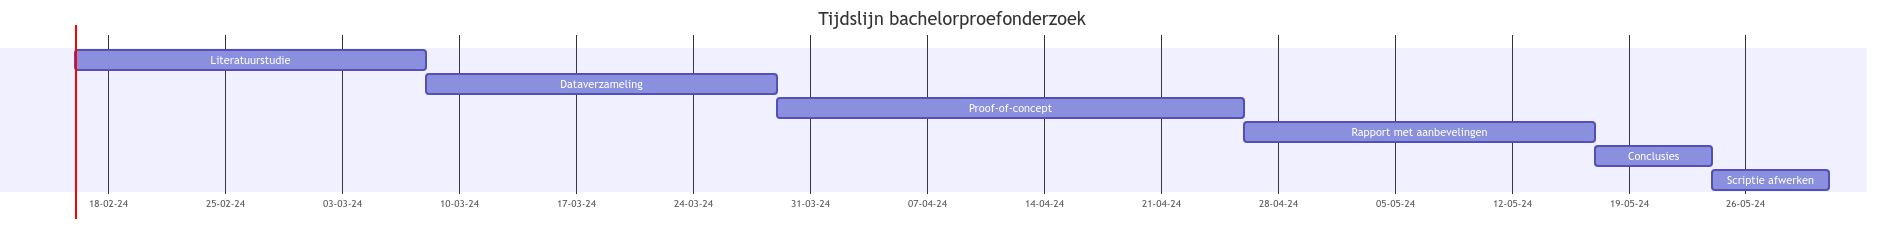
\includegraphics[width=0.5\textwidth]{ganttChart}

%---------- Verwachte resultaten ----------------------------------------------
\section{Verwacht resultaat}%
\label{sec:verwachte_resultaten}
Er wordt verwacht dat de resultaten uit de proof-of-concept zal leiden tot een bruikbaar rapport van aanbevelingen.
Deze aanbevelingen zullen concreet gesture-gebaseerde handelingen ter vervanging van de bestaande UI-gestuurde acties omvatten.
Voor elke aanbeveling zal er tevens ook een analyse op de gebruikservaringen tijdens het testen van de proof-of-concept aanwezig zijn.
De hypothese stelt dat het interageren met de digitale wereld met de getoetste gebruikersacties zal leiden tot een kortere tijdsduur dan bestaande UI-gestuurde ervaringen.

\section{Conclusie}%
\label{sec:conclusie}
Immersive AR en mobiele Augmented Reality hebben beiden hetzelfde doel: het toonbaar maken van digitale objecten op een weerspiegeling van de fysieke omgeving.
Toch maakt deze gelijkenis het niet voor de hand liggend om interacties met deze virtuele entiteiten op soortgelijke wijze te realiseren.
Dit rapport zal Tropos AR mogelijks kunnen helpen om haar bestaande klassieke user interface voor mobiele AR te kunnen vertalen naar haar Immersive tegenhanger met intu\"{\i}tieve gebaren.